\documentclass[letterpaper, 10pt]{article}

\usepackage[english]{custompack}
\usepackage{fullpage}
\usepackage{amssymb}
\usepackage{multicol}
\usepackage{mathtools}
%\usepackage{hyperref}
%\usepackage{abcproblem}
%\renewcommand{\thesubsection}{\alph{subsection}}

%\allowdisplaybreaks
%\numberwithin{theorem}{section}

\title{\textbf{Assignment 2}}
\author{Håkon Mork \\ ECSE 526 Artificial Intelligence}
\date{February 28, 2013}

\begin{document}
\maketitle
\noindent
\begin{multicols*}{2}

\section{Two-dimensional navigation}
\subsection{State utilities and optimal policy}
% (fold)
After 42 rounds of value iteration, the values converged to:
\[
	\begin{bmatrix}
		0.078 & 0.027 &       & -0.187 \\
		0.169 & 0.084 & 0.102 & -0.154 \\
		0.283 &       & 0.257 & -1 \\
		0.392 & 0.549 & 0.699 & 1
	\end{bmatrix}
\]
After 6 iterations, the optimal policy converged to:
\[
	\begin{bmatrix}
		\rightarrow & \downarrow &       & \leftarrow \\
		\downarrow & \rightarrow & \downarrow & \uparrow \\
		\downarrow &       & \downarrow &  \\
		\rightarrow & \rightarrow & \rightarrow & 
	\end{bmatrix}
\]
% (end)

\subsection{Linear algebra policy evaluation}
% (fold)
To construct the matrix $A$, observe that the final utility $b_{ij}$ in a given state $(i, j)$ on the board depends linearly on the utilities of its neighbors---and possibly itself, if the policy we've chosen causes us to face a wall and bounce back when we try to walk into it. 
For example, we have $u_{11} \gets r + 0.8 u_{11} + 0.2 u_{21}$ because going south will take us either south or west with $0.7$ and $0.1$ probability, respectively; thus going south from $(1,1)$ will make us bounce back to that same spot with probability $0.8$. 
On the other hand, going south from $(3,3)$ yields $u_{33} \gets r + 0.1 u_{23} + 0.7 u_{32} + 0.2 u_{43}$ as per the general rule, which applies when there are no obstacles present to obstruct movement, such as blocked squares or board boundaries. 

Following this line of reasoning, we can construct the $(16 \times 16)$ matrix $A$ whose entries are the weights by which the utility in each state depend on other states, following the format on page 657 of Russell and Norvig.
The entries in every row clearly have to sum to $1$, since every step we take must lead somewhere. 
%We can then repeatedly solve the linear system $A \mathbf{u}_n = \mathbf{u}_{n+1}$ until $\mathbf{u}_n = \mathbf{u}_{n+1}$. 
%Here, $\mathbf{u}_0$ is a zero vector apart from the terminal states $(4,1) = 1$ and $(4,2) = -1$. 
%The ``special'' states, i.e., the terminals $(4, 1)$ and $(4, 2)$ as well as the blocked squares $(2,2)$ and $(3, 4)$, are not influenced by any other squares, so they just retain their old value from one iteration to the next. 
%This is represented by these rows having a weight of $1$ on the corresponding column. 
Since the matrix is too big to fit here, please see appendix \ref{ssec:matrix}. 
It looks like policy iteration with both $r = -0.02$ and $r = -0.04$ converges to the same utility:
\[
\mathbf{b} = 
\begin{bmatrix}
	0.801 & 0.514 &       & -0.842 \\
	0.883 & 0.473 & 0.268 & -0.842 \\
	1     &       & 0.556 & -1     \\
	1     & 1     & 1     &  1
\end{bmatrix}
\]
This seems like a peculiar result; see appendix \ref{ssec:furthercomments} for further comments.

% \[
% \begin{bmatrix}
% 	 0.347 &  0.142 &        & -0.917 \\
% 	 0.434 &  0.141 &  0.095 & -0.888 \\
% 	 0.546 &        &  0.397 & -1     \\
% 	 0.575 &  0.675 &  0.825 &  1          
% \end{bmatrix}
% \]
% 
% \[
% \begin{bmatrix}
% 	-0.107 & -0.230 &        & -0.992 \\
% 	-0.015 & -0.191 & -0.079 & -0.935 \\
% 	 0.093 &        &  0.239 & -1     \\
% 	 0.150 &  0.350 &  0.650 &  1         
% \end{bmatrix}
% \]
% (end)

\subsection{State utilities are linear in $r$}
% (fold)
\begin{proof}
Consider equation 17.10 in Russell and Norvig:
\[ U_i(s) = R(s) + \gamma \sum_{s'} T(s, \pi_i(s), s') U_i(s') \]
The utility vector $\mathbf{u}$ consists of utilities such as this for all the states $s$ in the state space $\mathcal{S}$; that is, $\mathbf{u} = [U_i(s)]_{s \in \mathcal{S}}$.
We can then, by linearity of vector addition, split each $U_i$ into its constituent parts, one for the reward per state and one for the discounted utility of future state:
\begin{align*}
\mathbf{u} &= [U_i(s)]_{s \in \mathcal{S}} \\
&= \left[ R(s) + \gamma \sum_{s'} T(s, \pi_i(s), s') U_i(s') \right]_{s \in \mathcal{S}} \\
&= [R(s)]_{s \in \mathcal{S}} + \left[ \gamma \sum_{s'} T(s, \pi_i(s), s') U_i(s') \right]_{s \in \mathcal{S}} \\
&= r\mathbf{b} + \mathbf{c}
\end{align*}
where $[R(s)] = r\mathbf{b}$ since all states have a linear component of $r$ in their utility. 
Consider, for example, the vector
\[
\mathbf{b}[s] = \begin{dcases*}
0 & if state $s$ is a terminal \\
1 & otherwise
\end{dcases*}
\]
which I think accurately describes both our state space and those in the book.
\end{proof}
% (end)

% TODO
\subsection{Utility plot I}
% (fold)

% (end)

% TODO
\subsection{Utility plot II}
% (fold)
\begin{figure}[h]
	\centering
	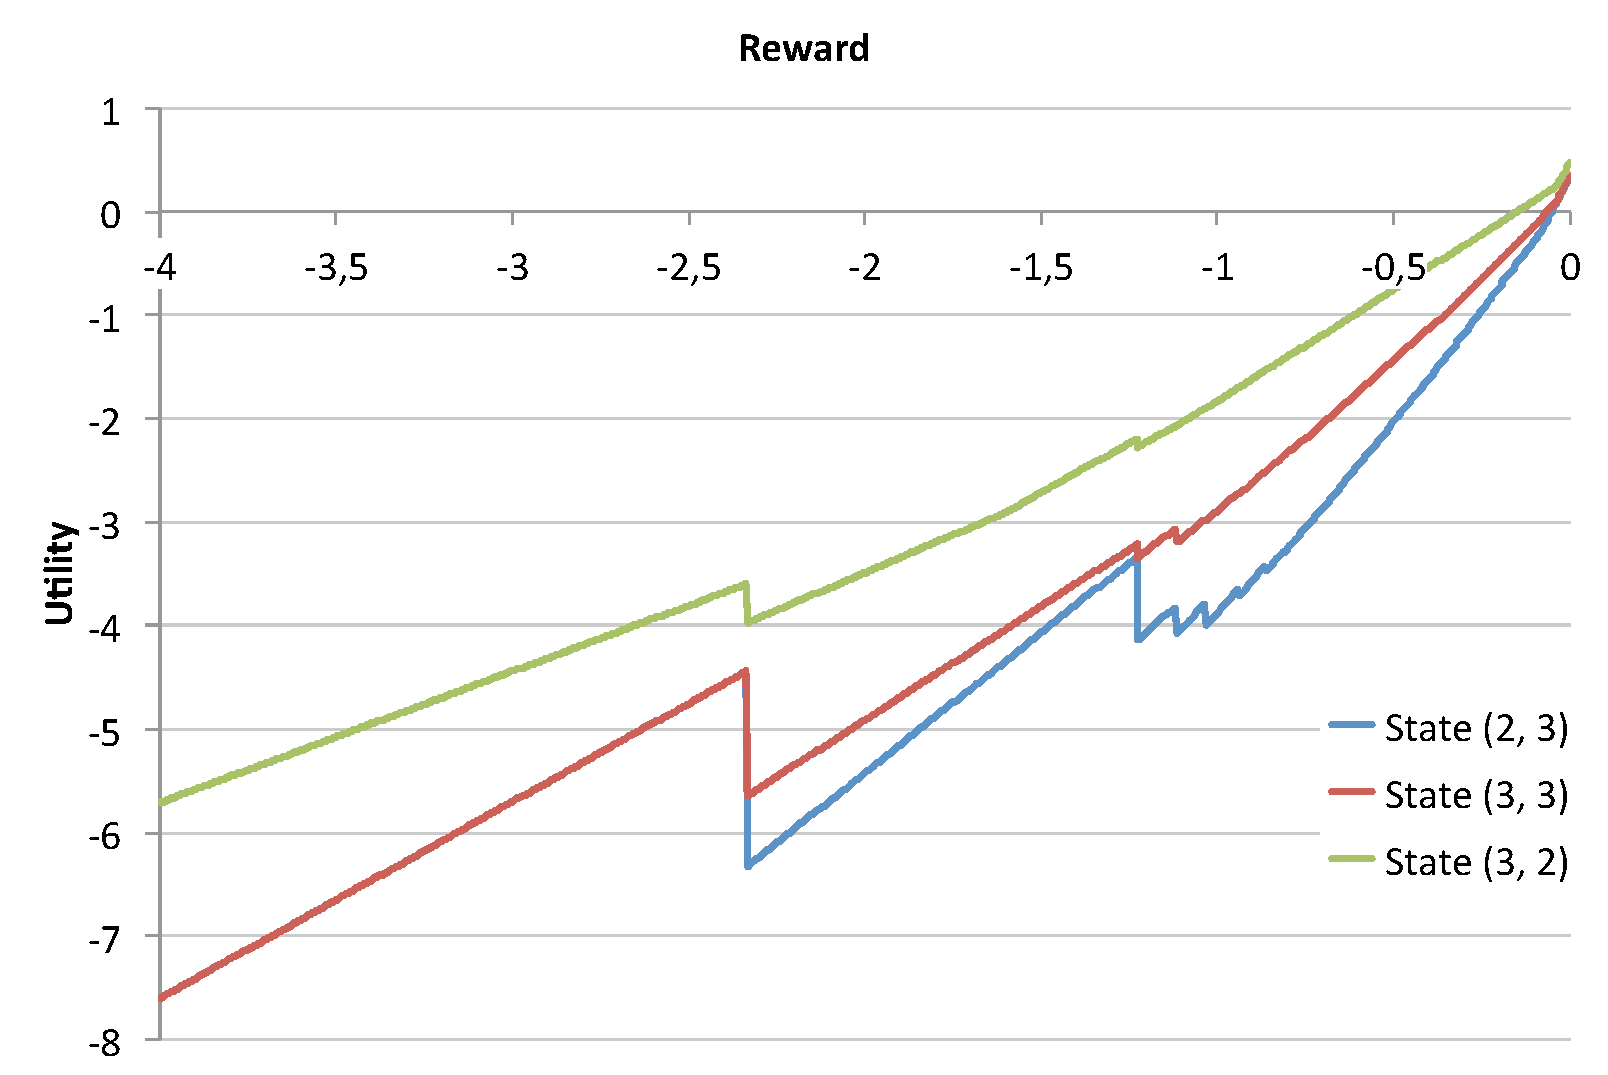
\includegraphics[width=0.3\textwidth]{prob15}
	\caption{}
	\label{fig:prob15}
\end{figure}
The utilities appear to be piecewise linear in $r$.
% (end)

% TODO
\subsection{Policy differences}
% (fold)
It would make sense for the optimal policy to change from a very negative $r$ to one closer to zero.
At $r = -3.5$, the agent is in a grim situation, and even jumping into the pit with utility $-1$ would be better than staying in the nonterminal squares and endure the penalty of a large negative $r$.
The less negative penalty of $r = -0.5$, on the other hand, may be sufficient for the agent to prefer going the long way around to the positive terminal node. 
% (end)

\subsection{Equation modification}
% (fold)
Equation 17.5 in Russell and Norvig is 
\[ U(s) = R(s) + \gamma \max_a \sum_{s'} T(s, a, s') U(s') \]
where we assume that the immediate reward $R(s)$ in state $s$ does not depend on what action we take; that is, $R(s) = R(s, a, s')$ for all $a$ and $s'$. 
%Note that 17.5 may be rewritten as 
%\[ U(s) = \gamma \max_a \left( \sum_{s'} T(s, a, s') U(s') + \frac{R(s)}{\gamma} \right)\]
%since $R(s)$ is independent of $a$.
If, however, the reward does depend on the action taken, the utility maximization over $a$ must extend to the reward as well, with the appropriate weighting $T$ for each direction. 
Therefore my guess is that we should write 
\[  U(s) = \gamma \max_a \sum_{s'} T(s, a, s') \left( U(s') + R(s, a, s') \right). \]
Still, this means that $R$ is discounted by $\gamma$ along with the utilities from neighboring states, which I'm not convinced is the right thing to do. 
%Maybe a multiplying $R$ by a factor $1/\gamma$ would work.
% (end)


\section{Feeding the kangaroo}
\subsection{State representation}
% (fold)
I see no reason not to represent the state space in the most straightforward way: as a one-dimensional array of utilities. 
I put the complexity of managing what states are terminals and not in the evaluation function. 
The convoluted jumping system is handled here too. 
% (end)

\subsection{Terminals and nonterminals}
% (fold)
We have three terminals: holes 3 and 7, and the food square 5. It also looks like we have \emph{seven} nonterminals: regular squares 1, 2, 4, 6, 8, and 9, as well as the food square 5: since the kangaroo has to perform a jump of magnitude zero to eat the food and win the game while standing in square 5, that square should be considered to be both a terminal and a nonterminal state. 
% (end)

\subsection{Possible actions}
% (fold)
\begin{tabular}{lcccccccccc}
	Jump & 1 & 2 & 3 & 4 & 5 & 6 & 7 & 8 & 9 \\
	\midrule
	2 left   & \checkmark & \checkmark & & \checkmark & & \checkmark & & \checkmark &  \\
	1 left   & \checkmark & \checkmark & & & \checkmark & \checkmark & & & \checkmark \\
	In place & \checkmark & \checkmark & & \checkmark & \checkmark & \checkmark & & \checkmark & \checkmark \\
	1 right  & \checkmark & & & \checkmark & \checkmark & & & \checkmark & \checkmark \\
	2 right  & & \checkmark & & \checkmark & & \checkmark & & \checkmark & \checkmark \\
\end{tabular}

\vspace{10pt}

\noindent 
I only consider actions that are ``allowed'' in the sense that we don't lose if we perform that action; for example, jumping one step to the right from square 2 would make the kangaroo tumble into the pit and lose, so that option is not considered feasible. I also consider squares 3 and 7 to be of little interest because being in one of them means that we've lost and the game is over, so it doesn't much matter what actions are possible there.
% (end)

% TODO
\subsection{State utilities and optimal policy}


\end{multicols*}
\clearpage
\appendix

\section{Linear algebra}
\subsection{The linear system from problem 1.2}
% (fold)
\label{ssec:matrix}
This is the system $A\mathbf{u} = \mathbf{b}$ from problem 1.2. Using the notation $\mathbf{u} = \mathbf{u}_n, \mathbf{b} = \mathbf{u}_{n+1}$, we can repeatedly solve the linear system $A \mathbf{u}_n = \mathbf{u}_{n+1}$ until convergence with $\mathbf{u}_n = \mathbf{u}_{n+1}$. I added lines in $A$ to identify $(4 \times 4)$ submatrices for the sake of readability. 
\[
% A
\left[
\begin{array}{cccc|cccc|cccc|cccc}
%11 & 12   & 13  & 14  & 21  & 22  & 23  & 24  & 31  & 32  & 33  & 34  & 41  & 42  & 43  & 44
0.8 & 0    & 0   & 0   & 0.2 & 0   & 0   & 0   & 0   & 0   & 0   & 0   & 0   & 0   & 0   & 0   \\ % 11
0.7 & 0.3  & 0   & 0   & 0   & 0   & 0   & 0   & 0   & 0   & 0   & 0   & 0   & 0   & 0   & 0   \\ % 12
0   & 0.7  & 0.1 & 0   & 0   & 0   & 0.2 & 0   & 0   & 0   & 0   & 0   & 0   & 0   & 0   & 0   \\ % 13
0   & 0    & 0.7 & 0.1 & 0   & 0   & 0   & 0.2 & 0   & 0   & 0   & 0   & 0   & 0   & 0   & 0   \\ % 14
\hline
0.1 & 0    & 0   & 0   & 0.7 & 0   & 0   & 0   & 0.2 & 0   & 0   & 0   & 0   & 0   & 0   & 0   \\ % 21
0   & 0    & 0   & 0   & 0   & 1   & 0   & 0   & 0   & 0   & 0   & 0   & 0   & 0   & 0   & 0   \\ % 22
0   & 0    & 0.1 & 0   & 0   & 0   & 0.7 & 0   & 0   & 0   & 0.2 & 0   & 0   & 0   & 0   & 0   \\ % 23
0   & 0    & 0   & 0.1 & 0   & 0   & 0.7 & 0.2 & 0   & 0   & 0   & 0   & 0   & 0   & 0   & 0   \\ % 24
\hline
0   & 0    & 0   & 0   & 0.1 & 0   & 0   & 0   & 0.7 & 0   & 0   & 0   & 0.2 & 0   & 0   & 0   \\ % 31
0   & 0    & 0   & 0   & 0   & 0   & 0   & 0   & 0.7 & 0.1 & 0   & 0   & 0   & 0.2 & 0   & 0   \\ % 32
0   & 0    & 0   & 0   & 0   & 0   & 0.1 & 0   & 0   & 0.7 & 0   & 0   & 0   & 0   & 0.2 & 0   \\ % 33
0   & 0    & 0   & 0   & 0   & 0   & 0   & 0   & 0   & 0   & 0   & 1   & 0   & 0   & 0   & 0   \\ % 34
\hline
0   & 0    & 0   & 0   & 0   & 0   & 0   & 0   & 0   & 0   & 0   & 0   & 1   & 0   & 0   & 0   \\ % 41
0   & 0    & 0   & 0   & 0   & 0   & 0   & 0   & 0   & 0   & 0   & 0   & 0   & 1   & 0   & 0   \\ % 42
0   & 0    & 0   & 0   & 0   & 0   & 0   & 0   & 0   & 0   & 0.1 & 0   & 0   & 0.7 & 0.2 & 0   \\ % 43
0   & 0    & 0   & 0   & 0   & 0   & 0   & 0   & 0   & 0   & 0   & 0   & 0   & 0   & 0.7 & 0.3    % 44
\end{array}
\right]
% u
\begin{bmatrix}
u_{11} \\
u_{12} \\
u_{13} \\
u_{14} \\
%\hline
u_{21} \\
u_{22} \\
u_{23} \\
u_{24} \\
%\hline
u_{31} \\
u_{32} \\
u_{33} \\
u_{34} \\
%\hline
u_{41} \\
u_{42} \\
u_{43} \\
u_{44}
\end{bmatrix}_n
\!\!\!
=
% b
\begin{bmatrix}
u_{11} \\
u_{12} \\
u_{13} \\
u_{14} \\
%\hline
u_{21} \\
u_{22} \\
u_{23} \\
u_{24} \\
%\hline
u_{31} \\
u_{32} \\
u_{33} \\
u_{34} \\
%\hline
u_{41} \\
u_{42} \\
u_{43} \\
u_{44}
\end{bmatrix}_{n+1}
\]
%We start with the initial vector $\mathbf{u}_0 = [r,r,r,r,r,r,r,r,r,r,r,r,1,-1,r,r]^T$, where $r$ is the reward, in our case $-0.04$.
% (end)

\subsection{Further comments} 
% (fold)
\label{ssec:furthercomments}
discuss adding r, augmented matrix
% (end)

\end{document}
